\begin{pa} \label{PA:2.3}
Let $f$ and $g$ be the functions defined by $f(t) = 2t^2$ and $g(t) = t^3 + 4t$.
\ba
	\item Determine $f'(t)$ and $g'(t)$.
	\item Let $p(t) = 2t^2 (t^3 + 4t)$ and observe that $p(t) = f(t) \cdot g(t)$.  Rewrite the formula for $p$ by distributing the $2t^2$ term.  Then, compute $p'(t)$ using the sum and constant multiple rules.
	\item True or false: $p'(t) = f'(t) \cdot g'(t)$.  
	\item Let $\ds q(t) = \frac{t^3 + 4t}{2t^2}$ and observe that $\ds q(t) = \frac{g(t)}{f(t)}$.  Rewrite the formula for $q$ by dividing each term in the numerator by the denominator and simplify to write $q$ as a sum of constant multiples of powers of $t$.  Then, compute $q'(t)$ using the sum and constant multiple rules.
	\item True or false: $\ds q'(t) = \frac{g'(t)}{f'(t)}$.  
\ea
%\begin{figure}[h]
%\begin{center}
%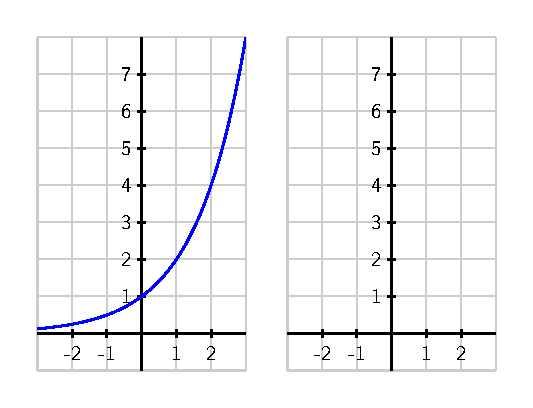
\includegraphics{figures/2_2_PA1a.eps}
%\caption{The graph of $y = g(x) = 2^x$.} \label{F:2.2.PA1}
%\end{center}
%\end{figure}

\end{pa} \afterpa